\documentclass[11pt]{report}

\usepackage[polish]{babel}
\usepackage{csquotes}
\DeclareQuoteAlias[]{dutch}{polish}
\usepackage{polski}
\usepackage{geometry}
\usepackage{listings}
\usepackage{xurl}
\usepackage{hyperref}
\usepackage{import}
\usepackage{multirow}
\usepackage{titling}
\usepackage{anyfontsize}
\usepackage[htt]{hyphenat}
\usepackage{xcolor}
\usepackage{graphicx}
\graphicspath{ {./EiWD_zadanie_03_wykresy/} }
\usepackage{subcaption}
\usepackage[
    style=numeric,
    sorting=nty,
    isbn=false,
    backend=biber, %biber EiWD_zadanie_03
]{biblatex}
\addbibresource{EiWD_zadanie_03.bib}

\newcommand{\prowadzacy}{prof. dr hab. inż. Vasyl Martsenyuk}
\newcommand{\temat}{Użycie biblioteki \enquote{PySpark} dla dużych zbiorów danych}
\newcommand{\wariant}{1}
\newcommand{\kierunek}{Informatyka}
\newcommand{\stopien}{II}
\newcommand{\tryb}{niestacjonarne}
\newcommand{\semestr}{III}
\newcommand{\grupa}{1}
\newcommand{\nrLab}{3}
\newcommand{\repozytorium}{https://colab.research.google.com/drive/102PjrGMDmssVFKQKxz3Sehfyq7MA4nKL?usp=sharing}

\definecolor{codegreen}{rgb}{0,0.6,0}
\definecolor{codegray}{rgb}{0.5,0.5,0.5}
\definecolor{codepurple}{rgb}{0.58,0,0.82}
\definecolor{backcolour}{rgb}{0.95,0.95,0.92}

\lstdefinestyle{mystyle}{
    backgroundcolor=\color{backcolour},   
    commentstyle=\color{codegreen},
    keywordstyle=\color{magenta},
    numberstyle=\tiny\color{codegray},
    stringstyle=\color{codepurple},
    basicstyle=\ttfamily\footnotesize,
    breakatwhitespace=false,         
    breaklines=true,                 
    captionpos=b,                    
    keepspaces=true,                 
    numbers=left,                    
    numbersep=5pt,                  
    showspaces=false,                
    showstringspaces=false,
    showtabs=false,                  
    tabsize=2
}

\lstset{style=mystyle}

\makeatletter
\renewcommand{\@makechapterhead}[1]{%
\vspace*{0 pt}%
{\setlength{\parindent}{0pt} \raggedright \normalfont
\bfseries\Huge\thechapter.\ #1
\par\nobreak\vspace{40 pt}}}
\makeatother

\newcounter{zadanie}
\newcommand{\zadanie}[1]{
    \refstepcounter{zadanie}
    \filbreak\vspace*{1cm}
    {\noindent\raggedright\Large \textbf{Zadanie~\thezadanie. #1}}
    \vspace{10 pt}\nopagebreak[1]
}

\begin{document}

\title{Eksploracja i wizualizacja danych}
\author{Piotr Rybka}
\date{24.11.2021}

\import{}{EiWD_title_page.tex}

\chapter*{Polecenie}

Na podstawie danych ze zbioru \cite{daneMedyczne} wypróbować podstawowe metody biblioteki \enquote{pyspark}.

\zadanie{Zainstalować pakiet \enquote{pyspark}}

Instalacja biblioteki w notatniku Google Colab (\url{https://research.google.com/colaboratory/}):

\begin{lstlisting}[language=Python]
!pip install pyspark==3.0.1 py4j==0.10.9
\end{lstlisting}

\zadanie{Utworzyć sesję \enquote{SparkSession}}

\begin{lstlisting}[language=Python]
from pyspark.sql import SparkSession

spark = SparkSession\
        .builder\
        .master('local[4]')\
        .appName('zadanie_4')\
        .getOrCreate()
\end{lstlisting}

\zadanie{Wczytać dane z pliku CSV i wyświetlić pierwsze 5 wierszy}

\begin{lstlisting}[language=Python]
csv_file = r"/content/IHME_DAH_DATABASE_1990_2020_Y2021M09D22.CSV"

data = spark.read.csv(csv_file, header=True)

# sposob 1
data.show(5)

# sposob 2
data.head(5)
\end{lstlisting}

Wynik działania obu funkcji: \ref{fig:wykres1} i \ref{fig:wykres2}.

\begin{figure}[h]
    \caption{Wynik działania funkcji \texttt{show()} (dane na podstawie \cite{daneMedyczne})}
    \label{fig:wykres1}
    \centering
    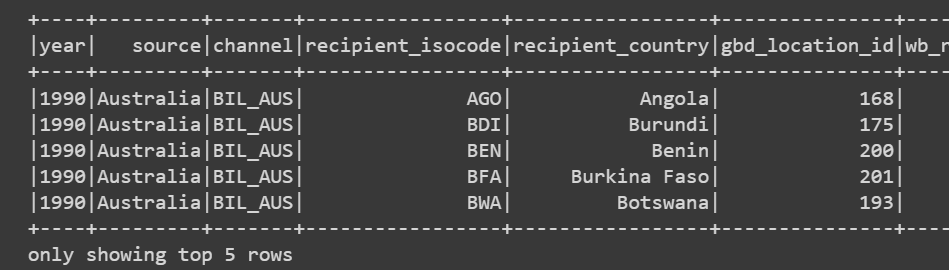
\includegraphics[width=.8\textwidth]{0001.png}
\end{figure}

\begin{figure}[h]
    \caption{Wynik działania funkcji \texttt{head()} (dane na podstawie \cite{daneMedyczne})}
    \label{fig:wykres2}
    \centering
    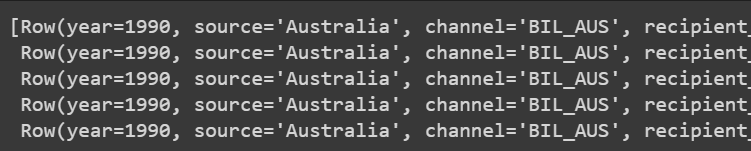
\includegraphics[width=.8\textwidth]{0002.png}
\end{figure}

\zadanie{Utworzyć schemat danych i zastosować go na zbiorze danych}

\begin{lstlisting}[language=Python]
# wyswietlenie pierwotnego schematu danych
data.printSchema()
    
from pyspark.sql.types import *

# utworzenie nowego schematu danych
data_schema = [
      StructField('year', IntegerType(), True),
      StructField('source', StringType(), True),
      StructField('channel', StringType(), True),
      StructField('recipient_isocode', StringType(), True),
      StructField('recipient_country', StringType(), True),
      StructField('gbd_location_id', IntegerType(), True),
      StructField('wb_regioncode', StringType(), True),
      StructField('wb_location_id', IntegerType(), True),
      StructField('gbd_region', StringType(), True),
      StructField('gbd_region_id', IntegerType(), True),
      StructField('gbd_superregion', StringType(), True),
      StructField('gbd_superregion_id', IntegerType(), True),
      StructField('elim_ch', IntegerType(), True),
      StructField('prelim_est', IntegerType(), True),
      StructField('dah_20', IntegerType(), True),
      StructField('rmh_fp_dah_20', IntegerType(), True),
      StructField('rmh_mh_dah_20', IntegerType(), True),
      StructField('rmh_hss_other_dah_20', IntegerType(), True),
      StructField('rmh_hss_hrh_dah_20', IntegerType(), True),
      StructField('rmh_other_dah_20', IntegerType(), True),
      StructField('nch_cnn_dah_20', IntegerType(), True),
      StructField('nch_cnv_dah_20', IntegerType(), True),
      StructField('nch_other_dah_20', IntegerType(), True),
      StructField('nch_hss_other_dah_20', IntegerType(), True),
      StructField('nch_hss_hrh_dah_20', IntegerType(), True),
      StructField('hiv_treat_dah_20', IntegerType(), True),
      StructField('hiv_prev_dah_20', IntegerType(), True),
      StructField('hiv_pmtct_dah_20', IntegerType(), True),
      StructField('hiv_other_dah_20', IntegerType(), True),
      StructField('hiv_ct_dah_20', IntegerType(), True),
      StructField('hiv_ovc_dah_20', IntegerType(), True),
      StructField('hiv_care_dah_20', IntegerType(), True),
      StructField('hiv_hss_other_dah_20', IntegerType(), True),
      StructField('hiv_hss_hrh_dah_20', IntegerType(), True),
      StructField('hiv_amr_dah_20', IntegerType(), True),
      StructField('mal_diag_dah_20', IntegerType(), True),
      StructField('mal_hss_other_dah_20', IntegerType(), True),
      StructField('mal_hss_hrh_dah_20', IntegerType(), True),
      StructField('mal_con_nets_dah_20', IntegerType(), True),
      StructField('mal_con_irs_dah_20', IntegerType(), True),
      StructField('mal_con_oth_dah_20', IntegerType(), True),
      StructField('mal_treat_dah_20', IntegerType(), True),
      StructField('mal_comm_con_dah_20', IntegerType(), True),
      StructField('mal_other_dah_20', IntegerType(), True),
      StructField('mal_amr_dah_20', IntegerType(), True),
      StructField('tb_other_dah_20', IntegerType(), True),
      StructField('tb_treat_dah_20', IntegerType(), True),
      StructField('tb_diag_dah_20', IntegerType(), True),
      StructField('tb_hss_other_dah_20', IntegerType(), True),
      StructField('tb_hss_hrh_dah_20', IntegerType(), True),
      StructField('tb_amr_dah_20', IntegerType(), True),
      StructField('oid_hss_other_dah_20', IntegerType(), True),
      StructField('oid_hss_hrh_dah_20', IntegerType(), True),
      StructField('oid_ebz_dah_20', IntegerType(), True),
      StructField('oid_zika_dah_20', IntegerType(), True),
      StructField('oid_covid_dah_20', IntegerType(), True),
      StructField('oid_other_dah_20', IntegerType(), True),
      StructField('oid_amr_dah_20', IntegerType(), True),
      StructField('ncd_hss_other_dah_20', IntegerType(), True),
      StructField('ncd_hss_hrh_dah_20', IntegerType(), True),
      StructField('ncd_tobac_dah_20', IntegerType(), True),
      StructField('ncd_mental_dah_20', IntegerType(), True),
      StructField('ncd_other_dah_20', IntegerType(), True),
      StructField('swap_hss_other_dah_20', IntegerType(), True),
      StructField('swap_hss_hrh_dah_20', IntegerType(), True),
      StructField('swap_hss_pp_dah_20', IntegerType(), True),
      StructField('other_dah_20', IntegerType(), True),
      StructField('rmh_dah_20', IntegerType(), True),
      StructField('nch_dah_20', IntegerType(), True),
      StructField('ncd_dah_20', IntegerType(), True),
      StructField('hiv_dah_20', IntegerType(), True),
      StructField('mal_dah_20', IntegerType(), True),
      StructField('tb_dah_20', IntegerType(), True),
      StructField('swap_hss_total_dah_20', IntegerType(), True),
      StructField('oid_dah_20', IntegerType(), True),
      StructField('unalloc_dah_20', IntegerType(), True),  
]

data_struc = StructType(fields = data_schema)

# dodanie schematu do danych
data2 = spark.read.csv(csv_file, header=True, schema=data_struc)

data2.printSchema()
\end{lstlisting}

Pierwotny schemat danych tuż po załadowaniu danych z plik CSV -- rys. \ref{fig:wykres3a} i po dodaniu schematu danych -- rys. \ref{fig:wykres3b}.

\begin{figure}[h]
    \begin{subfigure}{0.45\textwidth}
        \centering
        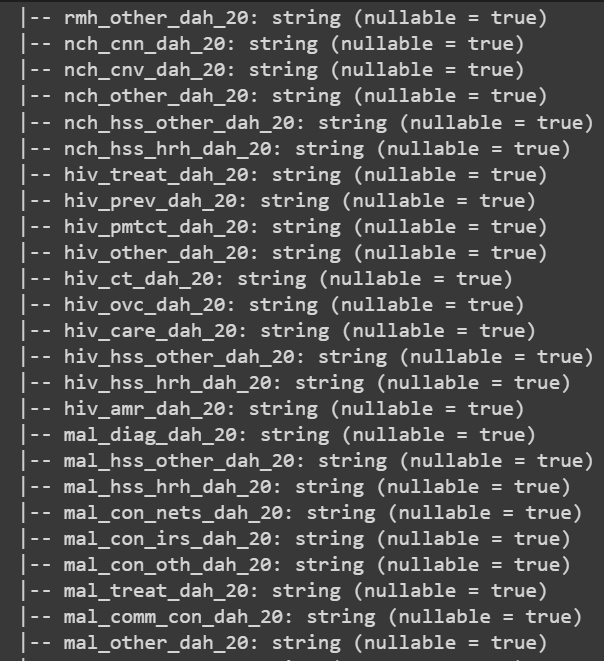
\includegraphics[width=.8\linewidth]{0003.png}
        \caption{Domyślny schemat danych}
        \label{fig:wykres3a}
    \end{subfigure}
    \begin{subfigure}{0.45\textwidth}
        \centering
        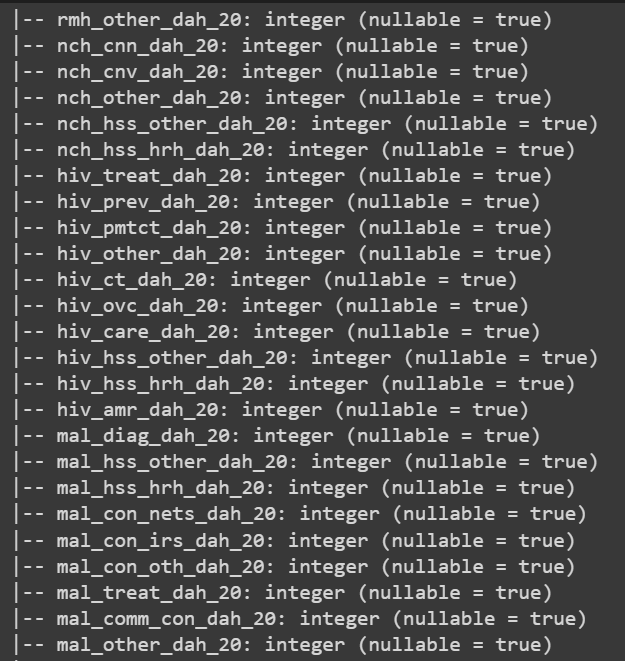
\includegraphics[width=.8\linewidth]{0004.png}
        \caption{Nowy schemat danych}
        \label{fig:wykres3b}
    \end{subfigure}
    \caption{Dane przed dodaniem i po dodaniu schematu danych (dane na podstawie \cite{daneMedyczne})}
    \label{fig:wykres3}
\end{figure}

\zadanie{Wyświetlić typy danych w poszczególnych kolumnach}

Funkcja:

\begin{lstlisting}[language=Python]
data.dtypes
\end{lstlisting}

Wynik działania funkcji -- rys. \ref{fig:wykres5}.

\begin{figure}[h]
    \caption{Typy danych (dane na podstawie \cite{daneMedyczne})}
    \label{fig:wykres5}
    \centering
    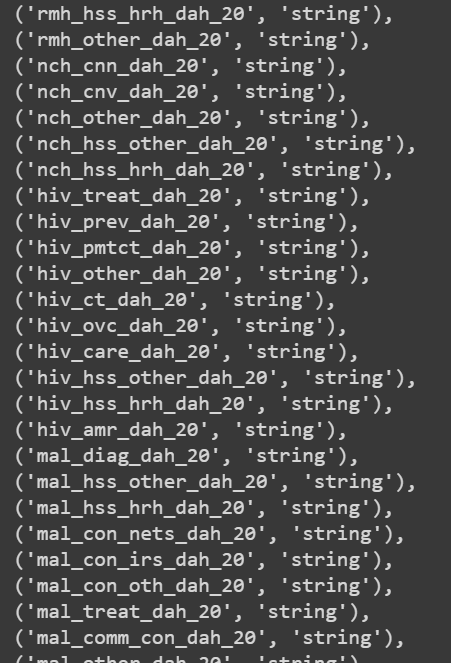
\includegraphics[width=.4\textwidth]{0005.png}
\end{figure}

\zadanie{Pokazać 2 pierwsze i ostatnie rekordy danych}

\begin{lstlisting}[language=Python]
data2.head(2)

data2.tail(2)
\end{lstlisting}

\zadanie{Dodać nową kolumnę zawierającą zera, zmienić jej nazwę, a następnie usunąć}

\begin{lstlisting}[language=Python]
# dodanie kolumny
res = data2.withColumn('Nowa kolumna', data2.year*0 + 1000)
    
# zmiana nazwy kolumny
res = res.withColumnRenamed('Nowa kolumna', 'col')

# usuniecie kolumny
res = data2.drop('col')
\end{lstlisting}

\zadanie{Dodać do danych kolumnę zawierającą numer wiersza}

\begin{lstlisting}[language=Python]
from pyspark.sql.functions import udf

# funkcja zwracajaca kolejne liczby naturalne od 0
i = -1
def incr():
    global i
    i = i+1
    return i

# utworzenie nowej kolumny
newCol = udf(incr, IntegerType())

# dodanie nowej kolumny
data3 = data2.withColumn('id', newCol())

data3.show(5)
\end{lstlisting}

Uzyskany wynik -- rys. \ref{fig:wykres6}

\begin{figure}[h]
    \caption{Dodatkowa kolumna z numerem wiersza (dane na podstawie \cite{daneMedyczne})}
    \label{fig:wykres6}
    \centering
    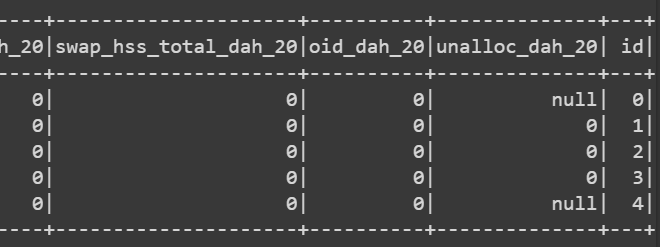
\includegraphics[width=.6\textwidth]{0006.png}
\end{figure}

\zadanie{Sprawdzić liczbę wierszy danych przed i po usunięciu wierszy bez danych dwoma sposobami}

\begin{lstlisting}[language=Python]
# poczatkowa liczba rekordow
data3.count()                   # wynik: 384 306

# usuniecie wierszy bez danych (sposob 1.)
data4 = data3.na.drop()

data4.count()                   # wynik: 136 560

# wstawienie zera w miejsce braku danych (sposob 2.)
data5 = data3.na.fill(data3.select(0 * data3.year).collect()[0][0])

data5.count()                   # wynik: 384 306
\end{lstlisting}

\zadanie{Wyświetlić wybrane kolumny danych}

\begin{lstlisting}[language=Python]
data5.select(['year', 'source', 'dah_20']).show(5)
\end{lstlisting}

Wyodrębnione kolumny -- rys.\ref{fig:wykres7}.

\begin{figure}[h]
    \caption{Pięć pierwszych wierszy wybranych kolumn danych (dane na podstawie \cite{daneMedyczne})}
    \label{fig:wykres7}
    \centering
    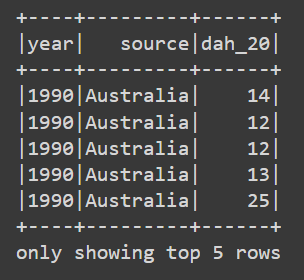
\includegraphics[width=.3\textwidth]{0007.png}
\end{figure}

\zadanie{Odfiltrować dane zawierające dane od roku 2000}

\begin{lstlisting}[language=Python]
from pyspark.sql.functions import col

data5.filter((col('year') >= 2000) & (col('dah_20') > 20)).select(['year', 'source', 'dah_20']).show(5)
\end{lstlisting}

Rezultat odfiltrowania danych -- rys. \ref{fig:wykres8}

\begin{figure}[h]
    \caption{Wynik filtrowania danych (rok 2000 i później, wartość \texttt{dah\_20} powyżej 20; dane na podstawie \cite{daneMedyczne})}
    \label{fig:wykres8}
    \centering
    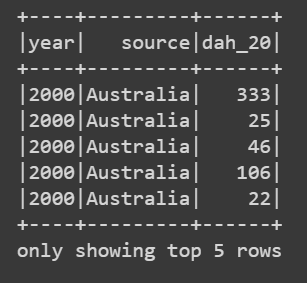
\includegraphics[width=.3\textwidth]{0008.png}
\end{figure}

\zadanie{Dodać kolumnę zawierającą wynik sprawdzenia warunku}

\begin{lstlisting}[language=Python]
# dodanie kolumny zawierajacej wynik sprawdzenia, czy rok jest wiekszy niz 2000
from pyspark.sql import functions as f

data5.select('year', 'source', 'dah_20', f.when(data5.year > 2000, '21st century').otherwise('20th century').alias('century')).show(5)

# dodanie kolumny zawierajacej wynik sprawdzenia, czy nazwa kraju zaczyna sie od litery 'A'
data5.select('year', 'source', 'dah_20', data5.source.rlike('^A').alias('A-country')).show(5)
\end{lstlisting}

Uzyskane dane -- rys. \ref{fig:wykres9} i

\begin{figure}[h]
    \caption{Nowa kolumna \texttt{century} zawierająca dane dyskretne (dane na podstawie \cite{daneMedyczne})}
    \label{fig:wykres9}
    \centering
    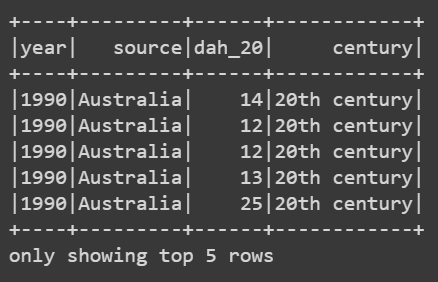
\includegraphics[width=.3\textwidth]{0009.png}
\end{figure}

\begin{figure}[h]
    \caption{Nowa kolumna \texttt{A-country} zawierająca dane typu logicznego (dane na podstawie \cite{daneMedyczne})}
    \label{fig:wykres10}
    \centering
    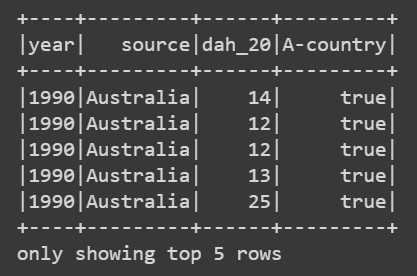
\includegraphics[width=.3\textwidth]{0010.png}
\end{figure}

\zadanie{Pogrupować dane wg kraju i obliczyć liczybę danych, średnią wartość oraz wartości minimalne i maksymalne}

\begin{lstlisting}[language=Python]
# pogrupowanie danych wg kraju
from pyspark.sql.functions import mean, count, min, max

data5\
    .select(['year', 'source', 'dah_20'])\
    .groupBy('source')\
    .agg(
        count('year').alias('number of countries'),
        mean('dah_20').alias('meah dah_20'),
        min('year').alias('min year'),
        max('year').alias('max year'),
    ).show(5)
\end{lstlisting}

Uzyskany wynik -- \ref{fig:wykres11}.

\begin{figure}[h]
    \caption{Przykład grupowania danych względem kolumny \texttt{source} (dane na podstawie \cite{daneMedyczne})}
    \label{fig:wykres11}
    \centering
    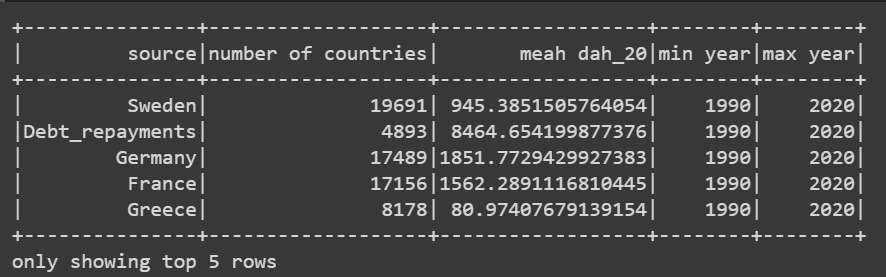
\includegraphics[width=.8\textwidth]{0011.png}
\end{figure}

\zadanie{Wygenerować wykres słupkowy na podstawie pogrupowanych danych}

\begin{lstlisting}[language=Python]
from matplotlib import pyplot as plt

res = data5\
    .filter(data5.source.rlike('^[ABC]'))\
    .select(['year', 'source', 'dah_20'])\
    .groupBy('source')\
    .agg(
        count('year').alias('number of countries'),
        mean('dah_20').alias('mean dah_20'),
        mean('year').alias('mean year'), 
        max('year').alias('max year'))\
    .toPandas()

res\
    .plot(kind='bar', x='source', y='number of countries')

plt.show()
\end{lstlisting}

Uzyskany wykres -- \ref{fig:wykres1}.

\begin{figure}[h]
    \caption{Wykres słupkowy liczby rekordów w wybranych krajach (dane na podstawie \cite{daneMedyczne})}
    \label{fig:wykres1}
    \centering
    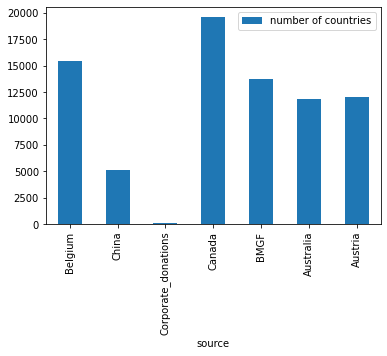
\includegraphics[width=.8\textwidth]{download}
\end{figure}

\chapter*{Wnioski}

Biblioteka \enquote{pyspark} jest wygodną alternatywą dla pakietu \enquote{pandas}, zwłaszcza jeśli analizowane są duże zbiory danych.

Wszelkie operacje na danych wymagają utworzenia sesji \enquote{SparkSession} przy użyciu biblioteki \texttt{builder}, np.

\begin{lstlisting}[language=Python]
from pyspark.sql import SparkSession

spark = SparkSession\
        .builder\
        .master('local[4]')\    # liczba rdzeni procesora
        .appName('zadanie')\    # nazwa sesji
        .getOrCreate()
\end{lstlisting}

Biblioteka \enquote{pyspark} pozwala wczytywać dane z różnych źródeł danych:

\begin{lstlisting}[language=Python]
# pliki CSV
data = spark.read.csv(csv_file_path, sep=',', header=True)

# pliki JSON
data = spark.read.json(json_data_file)

# pliki Parquet
data = spark.read.parquet(parquet_data_file)
\end{lstlisting}

Zapis wymaga użycia jednej z 2 funkcji:

\begin{lstlisting}[language=Python]
# pliki CSV
spark.write.csv(csv_file_path, sep=',', header=True)

# pliki JSON i Parquet
data = spark.write.save(json_data_file)
data = spark.write.save(parquet_data_file)
\end{lstlisting}

Wczytane dane są zwykle w formacie \enquote{string}, ale można nadarzucić im typ przy użyciu schematu, np.

\begin{lstlisting}[language=Python]
from pyspark.sql.types import *

data_schema = [
                StructField('Id', IntegerType(), False), 
                StructField('Miasto', StringType(), True), 
                StructField('Populacja', DoubleType(), True)
    ]
data_struc = StructType(fields = data_schema)

data = spark.read.csv(csv_file, sep=',', header=True, schema=data_struc)

# wyswietlenie schematu
data.printSchema()

# wyswietlenie typow danych
data.dtypes
\end{lstlisting}

Wybieranie wierszy odbywa się analogicznie jak w bibliotece \enquote{pandas}:

\begin{lstlisting}[language=Python]
data.head(1)        # pierwszy wiersz
data.show(1)        # jw.
data.tail(1)        # ostatni wiersz
\end{lstlisting}

Możliwe jest dodanie kolumny, zmiana jej nazwy oraz usunięcie, np.

\begin{lstlisting}[language=Python]
# dodanie kolumny
data = data.withColumn('Nowa kolumna', 1000000 + data.Id)

# zmiana nazwy kolumny
data = data.withColumnRenamed('Nowa kolumna', 'Id2')

# usuniecie kolumny
data = data.drop('Id2')
\end{lstlisting}

Wartości w nowych kolumnach można też dodawać przy użyciu osobnej funkcji, np.

\begin{lstlisting}[language=Python]
from pyspark.sql.functions import udf

i = -1
def incr():
  global i
  i = i+1
  return i

newCol = udf(incr, IntegerType())

csv_data = csv_data.withColumn('id', newCol())
\end{lstlisting}

Wiersze niezawierające danych mogą być łatwo usunięte na kilka sposobów:

\begin{itemize}
    \item przez zwykłe usunięcie wierszy:\\ \texttt{new\_data = data.na.drop()};
    \item przez wstawienie innych danych:\\ \texttt{new\_data = data.na.fill(data.select(data['kolumna']).collect()[0][0])};
    \item przez zastąpienie:\\ \texttt{new\_data = data.na.replace('stara wartosc', 'nowa wartosc')}.
\end{itemize}

Liczbę wierszy zwraca funkcja \texttt{data.count()}.

Istnieje kilka sposobów odwołania się do kolumny:

\begin{itemize}
    \item składnia kropkowa: \texttt{dane.kolumna} (nazwa kolumny nie może zawierać spacji);
    \item składnia indeksowa: \texttt{dane['kolumna']} (nazwa kolumny może być dowolna);
    \item funkcją \texttt{select}, podając jako jej parametr listę nazw kolumn, które mają być wyodrębnione.
\end{itemize}

Odfiltrowaniu danych służy funkcja \texttt{filter(c)}, zawierająca listę warunków połączonych spójnikami \verb|&| lub \verb-|-. Zakres danych można wskazać funkcją \texttt{dane.kolumna.between(a, b)}.

Wśród przydatnych funkcji w klasie \texttt{pyspark.sql.functions} można wymienić:

\begin{itemize}
    \item \texttt{udf(f, t)} -- pozwala zdefiniować kolumnę użytkownika i zapełnić ją danymi w typie \texttt{t} i zwracanymi przez funkcję \texttt{f};
    \item \texttt{mean(c)} -- średnia danych z kolumny \texttt{c};
    \item \texttt{col('nazwa')} -- kolumna, której wartości mają być porównywane;
    \item \texttt{when(c, a).otherwise(b)} -- zwraca wartość \texttt{a}, jeśli spełniony jest warunek \texttt{c} (w przeciwnym razie zwracane jest \texttt{b});
    \item \texttt{dane.kolumna.rlike(regex)} -- zwraca \texttt{true}, jeśli wartość w wierszu kolumny pasuje do wyrażenia regularnego.
\end{itemize}

Nazwy kolumn można aliasować funkcją \texttt{dane.kolumna.alias('nowa nazwa')}.

Grupowanie odbywa się przez użycie funkcji \texttt{groupBy}, przyjmującej listę kolumn, względem któych dane mają być pogrupowane. Funkcja \texttt{agg} pozwala przekazać funkcje agregujące dane z przekazanych im kolumn.

\begin{center}
    \texttt{dane.select(['kol1']).groupBy('kol1').agg(f1('kol2'), f2('kol3'))}
\end{center}

Funkcją \texttt{toPandas()} można każdy zbiór danych przekształcić do ramki danych, którą z kolei można przetwarzać przy użyciu biblioteki \texttt{pandas} i innych.


%\cleardoublepage

\printbibliography[heading=subbibliography,title={Strony internetowe},keyword=www]

\end{document}